\section{Dashboard I: Improve student engagement with the platform and optimize student learning through personalization}

The subgoals of this dashboard are to not lose the user's engagement with 
the platform and to help in adapting the learning process to the user's
needs. 

To make the user aware that he/she is looking
at the home page of the platform is added the name \textit{OffSec},
which states for \textit{Offensive Cybersecurity}, that is the field
in which the user has to upskill his/her expertise. To remark that this
dashboard is the home page is added \textit{Welcome Marta!} message.
These two elements help the user to not use the wrong mental model
when he/she has to interpret the elements present inside the dashboard.
In this way, the \textbf{Wrong Mental Model} demon is avoided.


\begin{figure}[H]
    \centering
    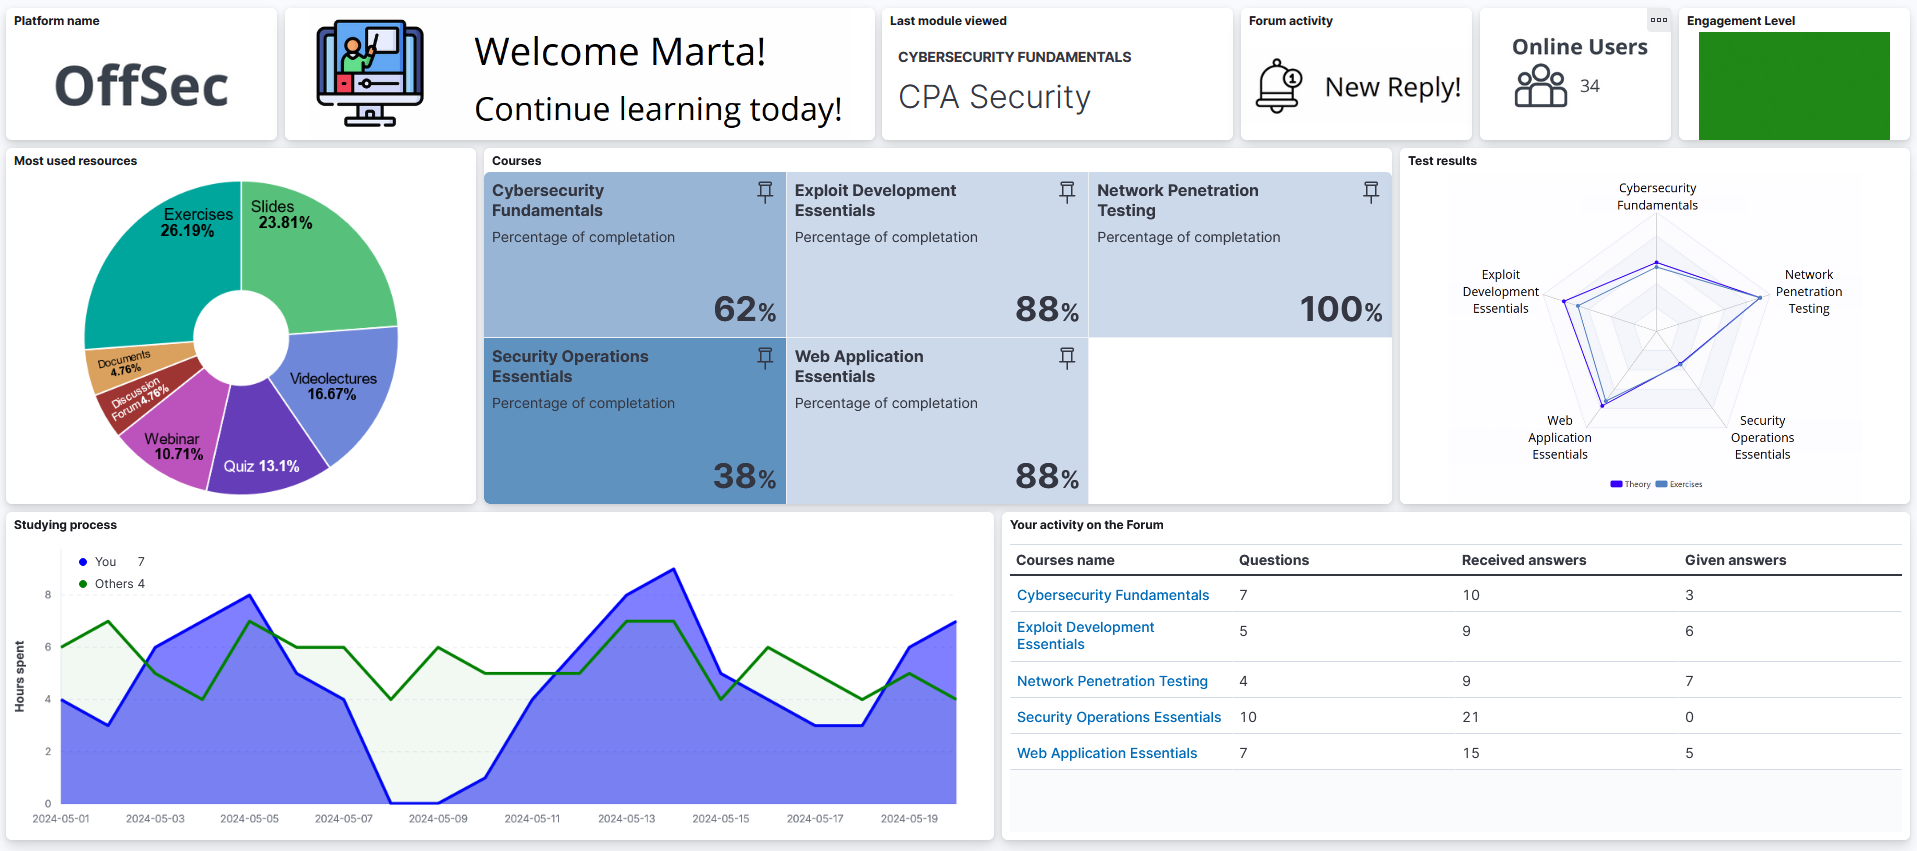
\includegraphics[width=0.9\textwidth]{assets/dashboard_1.png}
    \caption{Dashboard I}
    \label{fig:dashboard_1}
\end{figure}

Going more in detail about which elements present in the dashboard 
ensure the persue of the goals and which ensure the global situation
of the student. The \textbf{subgoal 1.2.1} is guaranteed by the linear graph,
which shows the user's time spent on the platform since the start of
the process of upskill, and by the table containing the activity of the
user on the forum, showing how many questions the user asked, how many
answers received and how many answers the user has given. 
Both the elements are shown in the following figure.

\begin{figure}[H]
    \centering
    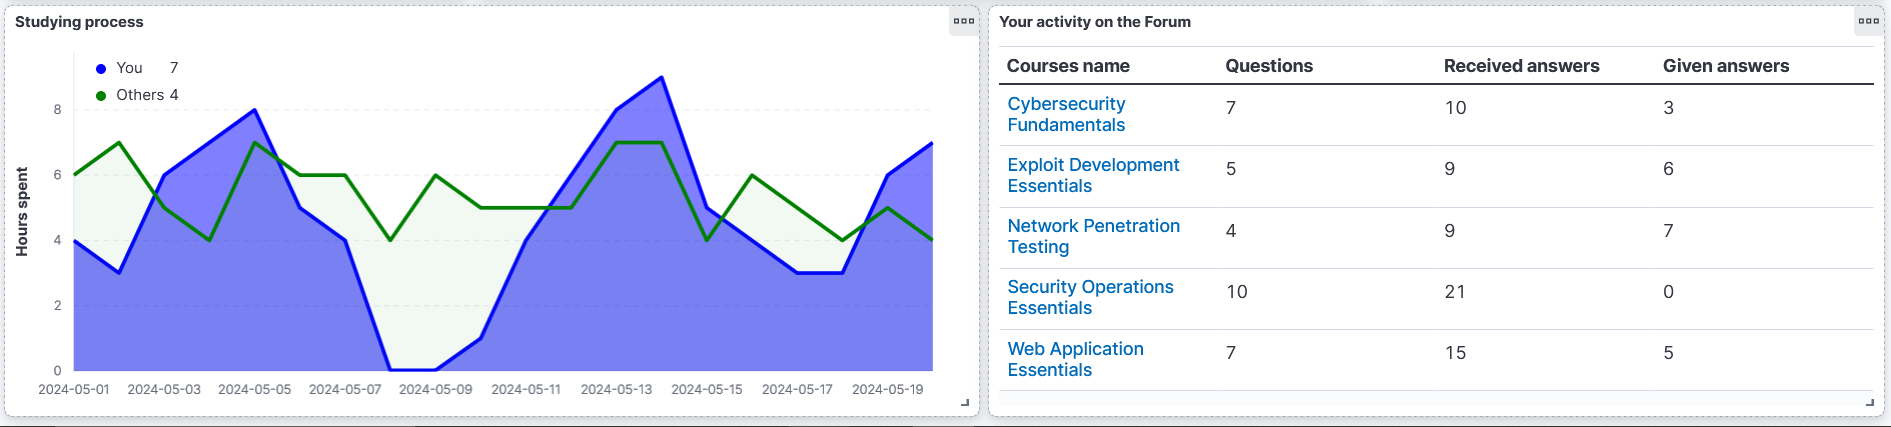
\includegraphics[width=0.9\textwidth]{assets/dashboard_1_121.png}
    \caption{Dashboard I - Subgoal 1.2.1}
    \label{fig:dashboard_1_subgoal_121}
\end{figure}


The \textbf{subgoal 1.2.2} is guaranteed by the donut chart, which shows how much
of the different resources are available for the different course the user has
used. The other element contributing to this subgoal is the matrix containing
the different courses the user has to complete in order to upskill himself/herself,
in this matrix is shown the percentage of completion of each course. These elements
are shown in the following figure.

\begin{figure}[H]
    \centering
    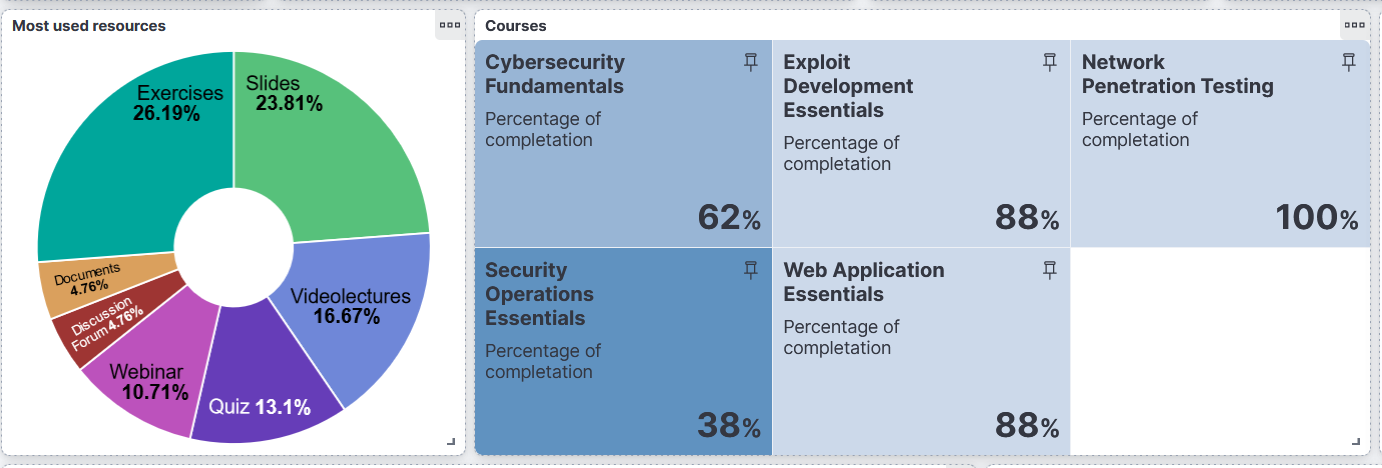
\includegraphics[width=0.9\textwidth]{assets/dashboard_1_122.png}
    \caption{Dashboard I - Subgoal 1.2.2}
    \label{fig:dashboard_1_subgoal_122}
\end{figure}

The four elements described above occupy the majority of the dashboard on 
the left side of the screen allowing the user to have a clear and complete
understanding of his/her engagement with the platform and how he/she has to
adapt his/her learning path, hence supporting the user's goals. 

The remaining part of the dashboard, following the
\textbf{Principle 4}, contains different elements that remind the user his/her
situation regarding the subgoals of the first major goal (how he/she is upgrading 
his/her skill). 

\begin{figure}[H]
    \centering
    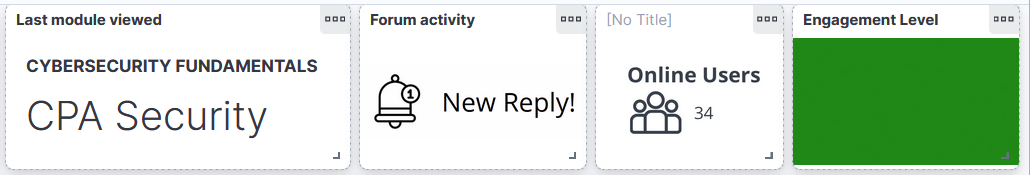
\includegraphics[width=0.9\textwidth]{assets/dashboard_1_globaltop.png}
    \caption{Dashboard I - Global Top}
    \label{fig:dashboard_1_global_top}
\end{figure}

These elements show user engagement with the platform by showing (from right to left)
the level of engagement computed with the CST (top-right),
how many users are online (top-right), a section
where are shown notifications from the forum (top-center). 
And an element where is present the last viewed module (top-center) which helps the user
to remember what module studied as last.
All these elements ensure to have the global situation awareness in each moment, 
to avoid the \textbf{Attentional Tunneling} demon. The user is not only focused
on his/her engagement with the platform or his/her state in the learning process, but is
also aware of his/her results from all the tests he/she has done until now.

For this dashboard, the \textbf{Principle 1}, the \textbf{Principle 2} and the \textbf{Principle 3},
have been used as base principles to design the different elements. Thanks to that, the 
visualization of the user's goal is easy to find, since the elements are positioned in center-left
part of the screen. 

In order to support the user's comprehension and avoid the 
\textbf{Memory Trap} demon, the data are processed and integrated: the spider chart
(positioned on the right side) shows in a faster way the results of the user than
could be done with a table. For the same reason, the donut chart allows a clearer 
understanding of which resources the user prefers more. This kind of visualization of the
data helps in reducing the quantity of data to show in the dashboard, in order to 
avoid the \textbf{Data Overload} demon. Consequentely, the \textbf{Complexity Creep} demon is not present.

Regarding level three of
Situation Awareness, the linear graph helps the user to project the time he/she will
spend on the platform in the future on the base of the actual trend.

